% Options for packages loaded elsewhere
\PassOptionsToPackage{unicode}{hyperref}
\PassOptionsToPackage{hyphens}{url}
\PassOptionsToPackage{dvipsnames,svgnames,x11names}{xcolor}
%
\documentclass[
]{ltjsarticle}

\usepackage{amsmath,amssymb}
\usepackage{iftex}
\ifPDFTeX
  \usepackage[T1]{fontenc}
  \usepackage[utf8]{inputenc}
  \usepackage{textcomp} % provide euro and other symbols
\else % if luatex or xetex
  \usepackage{unicode-math}
  \defaultfontfeatures{Scale=MatchLowercase}
  \defaultfontfeatures[\rmfamily]{Ligatures=TeX,Scale=1}
\fi
\usepackage{lmodern}
\ifPDFTeX\else  
    % xetex/luatex font selection
\fi
% Use upquote if available, for straight quotes in verbatim environments
\IfFileExists{upquote.sty}{\usepackage{upquote}}{}
\IfFileExists{microtype.sty}{% use microtype if available
  \usepackage[]{microtype}
  \UseMicrotypeSet[protrusion]{basicmath} % disable protrusion for tt fonts
}{}
\makeatletter
\@ifundefined{KOMAClassName}{% if non-KOMA class
  \IfFileExists{parskip.sty}{%
    \usepackage{parskip}
  }{% else
    \setlength{\parindent}{0pt}
    \setlength{\parskip}{6pt plus 2pt minus 1pt}}
}{% if KOMA class
  \KOMAoptions{parskip=half}}
\makeatother
\usepackage{xcolor}
\setlength{\emergencystretch}{3em} % prevent overfull lines
\setcounter{secnumdepth}{-\maxdimen} % remove section numbering

\usepackage{color}
\usepackage{fancyvrb}
\newcommand{\VerbBar}{|}
\newcommand{\VERB}{\Verb[commandchars=\\\{\}]}
\DefineVerbatimEnvironment{Highlighting}{Verbatim}{commandchars=\\\{\}}
% Add ',fontsize=\small' for more characters per line
\usepackage{framed}
\definecolor{shadecolor}{RGB}{241,243,245}
\newenvironment{Shaded}{\begin{snugshade}}{\end{snugshade}}
\newcommand{\AlertTok}[1]{\textcolor[rgb]{0.68,0.00,0.00}{#1}}
\newcommand{\AnnotationTok}[1]{\textcolor[rgb]{0.37,0.37,0.37}{#1}}
\newcommand{\AttributeTok}[1]{\textcolor[rgb]{0.40,0.45,0.13}{#1}}
\newcommand{\BaseNTok}[1]{\textcolor[rgb]{0.68,0.00,0.00}{#1}}
\newcommand{\BuiltInTok}[1]{\textcolor[rgb]{0.00,0.23,0.31}{#1}}
\newcommand{\CharTok}[1]{\textcolor[rgb]{0.13,0.47,0.30}{#1}}
\newcommand{\CommentTok}[1]{\textcolor[rgb]{0.37,0.37,0.37}{#1}}
\newcommand{\CommentVarTok}[1]{\textcolor[rgb]{0.37,0.37,0.37}{\textit{#1}}}
\newcommand{\ConstantTok}[1]{\textcolor[rgb]{0.56,0.35,0.01}{#1}}
\newcommand{\ControlFlowTok}[1]{\textcolor[rgb]{0.00,0.23,0.31}{#1}}
\newcommand{\DataTypeTok}[1]{\textcolor[rgb]{0.68,0.00,0.00}{#1}}
\newcommand{\DecValTok}[1]{\textcolor[rgb]{0.68,0.00,0.00}{#1}}
\newcommand{\DocumentationTok}[1]{\textcolor[rgb]{0.37,0.37,0.37}{\textit{#1}}}
\newcommand{\ErrorTok}[1]{\textcolor[rgb]{0.68,0.00,0.00}{#1}}
\newcommand{\ExtensionTok}[1]{\textcolor[rgb]{0.00,0.23,0.31}{#1}}
\newcommand{\FloatTok}[1]{\textcolor[rgb]{0.68,0.00,0.00}{#1}}
\newcommand{\FunctionTok}[1]{\textcolor[rgb]{0.28,0.35,0.67}{#1}}
\newcommand{\ImportTok}[1]{\textcolor[rgb]{0.00,0.46,0.62}{#1}}
\newcommand{\InformationTok}[1]{\textcolor[rgb]{0.37,0.37,0.37}{#1}}
\newcommand{\KeywordTok}[1]{\textcolor[rgb]{0.00,0.23,0.31}{#1}}
\newcommand{\NormalTok}[1]{\textcolor[rgb]{0.00,0.23,0.31}{#1}}
\newcommand{\OperatorTok}[1]{\textcolor[rgb]{0.37,0.37,0.37}{#1}}
\newcommand{\OtherTok}[1]{\textcolor[rgb]{0.00,0.23,0.31}{#1}}
\newcommand{\PreprocessorTok}[1]{\textcolor[rgb]{0.68,0.00,0.00}{#1}}
\newcommand{\RegionMarkerTok}[1]{\textcolor[rgb]{0.00,0.23,0.31}{#1}}
\newcommand{\SpecialCharTok}[1]{\textcolor[rgb]{0.37,0.37,0.37}{#1}}
\newcommand{\SpecialStringTok}[1]{\textcolor[rgb]{0.13,0.47,0.30}{#1}}
\newcommand{\StringTok}[1]{\textcolor[rgb]{0.13,0.47,0.30}{#1}}
\newcommand{\VariableTok}[1]{\textcolor[rgb]{0.07,0.07,0.07}{#1}}
\newcommand{\VerbatimStringTok}[1]{\textcolor[rgb]{0.13,0.47,0.30}{#1}}
\newcommand{\WarningTok}[1]{\textcolor[rgb]{0.37,0.37,0.37}{\textit{#1}}}

\providecommand{\tightlist}{%
  \setlength{\itemsep}{0pt}\setlength{\parskip}{0pt}}\usepackage{longtable,booktabs,array}
\usepackage{calc} % for calculating minipage widths
% Correct order of tables after \paragraph or \subparagraph
\usepackage{etoolbox}
\makeatletter
\patchcmd\longtable{\par}{\if@noskipsec\mbox{}\fi\par}{}{}
\makeatother
% Allow footnotes in longtable head/foot
\IfFileExists{footnotehyper.sty}{\usepackage{footnotehyper}}{\usepackage{footnote}}
\makesavenoteenv{longtable}
\usepackage{graphicx}
\makeatletter
\def\maxwidth{\ifdim\Gin@nat@width>\linewidth\linewidth\else\Gin@nat@width\fi}
\def\maxheight{\ifdim\Gin@nat@height>\textheight\textheight\else\Gin@nat@height\fi}
\makeatother
% Scale images if necessary, so that they will not overflow the page
% margins by default, and it is still possible to overwrite the defaults
% using explicit options in \includegraphics[width, height, ...]{}
\setkeys{Gin}{width=\maxwidth,height=\maxheight,keepaspectratio}
% Set default figure placement to htbp
\makeatletter
\def\fps@figure{htbp}
\makeatother

\makeatletter
\@ifpackageloaded{tcolorbox}{}{\usepackage[skins,breakable]{tcolorbox}}
\@ifpackageloaded{fontawesome5}{}{\usepackage{fontawesome5}}
\definecolor{quarto-callout-color}{HTML}{909090}
\definecolor{quarto-callout-note-color}{HTML}{0758E5}
\definecolor{quarto-callout-important-color}{HTML}{CC1914}
\definecolor{quarto-callout-warning-color}{HTML}{EB9113}
\definecolor{quarto-callout-tip-color}{HTML}{00A047}
\definecolor{quarto-callout-caution-color}{HTML}{FC5300}
\definecolor{quarto-callout-color-frame}{HTML}{acacac}
\definecolor{quarto-callout-note-color-frame}{HTML}{4582ec}
\definecolor{quarto-callout-important-color-frame}{HTML}{d9534f}
\definecolor{quarto-callout-warning-color-frame}{HTML}{f0ad4e}
\definecolor{quarto-callout-tip-color-frame}{HTML}{02b875}
\definecolor{quarto-callout-caution-color-frame}{HTML}{fd7e14}
\makeatother
\makeatletter
\@ifpackageloaded{caption}{}{\usepackage{caption}}
\AtBeginDocument{%
\ifdefined\contentsname
  \renewcommand*\contentsname{Table of contents}
\else
  \newcommand\contentsname{Table of contents}
\fi
\ifdefined\listfigurename
  \renewcommand*\listfigurename{List of Figures}
\else
  \newcommand\listfigurename{List of Figures}
\fi
\ifdefined\listtablename
  \renewcommand*\listtablename{List of Tables}
\else
  \newcommand\listtablename{List of Tables}
\fi
\ifdefined\figurename
  \renewcommand*\figurename{図}
\else
  \newcommand\figurename{図}
\fi
\ifdefined\tablename
  \renewcommand*\tablename{Table}
\else
  \newcommand\tablename{Table}
\fi
}
\@ifpackageloaded{float}{}{\usepackage{float}}
\floatstyle{ruled}
\@ifundefined{c@chapter}{\newfloat{codelisting}{h}{lop}}{\newfloat{codelisting}{h}{lop}[chapter]}
\floatname{codelisting}{Listing}
\newcommand*\listoflistings{\listof{codelisting}{List of Listings}}
\makeatother
\makeatletter
\makeatother
\makeatletter
\@ifpackageloaded{caption}{}{\usepackage{caption}}
\@ifpackageloaded{subcaption}{}{\usepackage{subcaption}}
\makeatother
\ifLuaTeX
  \usepackage{selnolig}  % disable illegal ligatures
\fi
\usepackage{bookmark}

\IfFileExists{xurl.sty}{\usepackage{xurl}}{} % add URL line breaks if available
\urlstyle{same} % disable monospaced font for URLs
\hypersetup{
  pdftitle={Quarto はじめて良かったこと},
  pdfauthor={司馬博文},
  colorlinks=true,
  linkcolor={blue},
  filecolor={Maroon},
  citecolor={Blue},
  urlcolor={minty},
  pdfcreator={LaTeX via pandoc}}

%\PassOptionsToPackage{top=15truemm,bottom=15truemm,left=10truemm,right=10truemm}{geometry}
\usepackage[top=15truemm,bottom=15truemm,left=10truemm,right=10truemm]{geometry}
\usepackage{picture}
\usepackage{fontawesome5}
\definecolor{minty}{HTML}{80c4ac}\definecolor{花緑青}{cmyk}{1,0.07,0.10,0.10}\definecolor{ISMBlue}{HTML}{2F579C}

% \titleformat{\subsection}[block]
% {}{}{0pt}
% {
%     \colorbox{minty}{\begin{picture}(0,10)\end{picture}}
%     \hspace{0pt}
%     \normalfont \Large\bfseries
%     \hspace{-4pt}
% }
% [
% \begin{picture}(100,0)
%     \put(3,18){\color{minty}\line(1,0){300}}
% \end{picture}
% \\
% \vspace{-30pt}
% ]

% \titlespacing{\subsection}{0pc}{3.5ex plus .1ex minus .2ex}{1.5ex minus .1ex}

% \renewcommand{\labelitemi}{\textcolor{minty}{\faCheckCircle}} %https://mirrors.ibiblio.org/CTAN/fonts/fontawesome/doc/fontawesome.pdf
% \faPaperclip が文献の列挙に良いかも.

\usepackage{comment}
\usepackage{mathtools} %内部でamsmathを呼び出すことに注意.
\usepackage{amsfonts} %mathfrak, mathcal, mathbbなど.
\usepackage{amsthm} %定理環境.
\usepackage{amssymb} %AMSFontsを使うためのパッケージ.
\usepackage{ascmac} %screen, itembox, shadebox環境.全てLATEX2εの標準機能の範囲で作られたもの.
\def\objectstyle{\displaystyle}
% \usepackage{xeCJK}  % ダウンロード長すぎる
% \setCJKmainfont{UDEVGothicNF-Regular.ttf}  % UDEVGothicNF-Regular.ttf が使いたい
% \usepackage{luatexja-fontspec}
% \setmainfont{みかちゃん.ttf}  % 英語だけ動いた.何?
\usepackage{enumerate} %enumerate環境を凝らせる.
\renewcommand{\labelenumi}{(\arabic{enumi})} %(1),(2),...がデフォルトであって欲しい
\renewcommand{\labelenumii}{(\roman{enumii})}
\renewcommand{\labelenumiii}{(\alph{enumiii})}
\usepackage{luatexja}
\usepackage{footnote}\title{Quarto はじめて良かったこと}
\author{司馬博文}
\date{11/04/2023}

\begin{document}
\maketitle
\begin{abstract}
Quarto は TeX
のような使用感で,数式とコードが併存する文章を書き,1つのソースファイルから
PDF, HTML, Word, Reveal.js, PowerPoint
などの多様な形式に出力できる次世代の執筆環境である.TeX, RStudio,
Jupyter Notebook のいずれかに慣れている人であれば,極めて手軽に Quarto
を使うことができる.筆者が用意した テンプレート
から簡単に始めることができる.
\end{abstract}

\subsection{使い方の概要}\label{ux4f7fux3044ux65b9ux306eux6982ux8981}

\subsubsection{導入}\label{ux5c0eux5165}

本サイトは Quarto と,GitHub Actions によってホスティングされている.

\begin{tcolorbox}[enhanced jigsaw, bottomrule=.15mm, leftrule=.75mm, colframe=quarto-callout-important-color-frame, opacityback=0, toprule=.15mm, colback=white, arc=.35mm, breakable, rightrule=.15mm, left=2mm]

\begin{itemize}
\tightlist
\item
  \href{../../2024/Process/Levy.qmd}{Lévy 過程を見てみよう}
  など,コードと数式を併せて書いている Jupyter Notebook のようなページ
\item
  \href{../../../static/CV/cv.qmd}{CV} など,HTML と PDF
  の両方で見れるページ
\item
  \href{../../2024/Slides/ZigZagSampler.qmd}{Zig-Zag サンプラー}
  など,HTML とスライド (reveal.js) の両方で見れるページ
\item
  本ページなど,HTML とスライド (pptx),typst PDF と LaTeX PDF と
  reveal.js のさまざまで見れるページ
\end{itemize}

\end{tcolorbox}

\begin{tcolorbox}[enhanced jigsaw, bottomrule=.15mm, leftrule=.75mm, colframe=quarto-callout-important-color-frame, opacityback=0, toprule=.15mm, colback=white, arc=.35mm, breakable, rightrule=.15mm, left=2mm]

\vspace{-3mm}\textbf{注}\vspace{3mm}

スマホでは別フォーマットのページのリンクは表示されないようである.

\end{tcolorbox}

\begin{Shaded}
\begin{Highlighting}[]
\ImportTok{using} \BuiltInTok{Plots}

\NormalTok{p }\OperatorTok{=} \FunctionTok{plot}\NormalTok{(sin, }
     \FunctionTok{x{-}\textgreater{}sin}\NormalTok{(}\FloatTok{2}\NormalTok{x), }
     \FloatTok{0}\NormalTok{, }
     \FloatTok{2}\NormalTok{π, }
\NormalTok{     leg}\OperatorTok{=}\ConstantTok{false}\NormalTok{, }
\NormalTok{     fill}\OperatorTok{=}\NormalTok{(}\FloatTok{0}\NormalTok{,}\OperatorTok{:}\NormalTok{lavender))}
\end{Highlighting}
\end{Shaded}

\begin{figure}[H]

\centering{

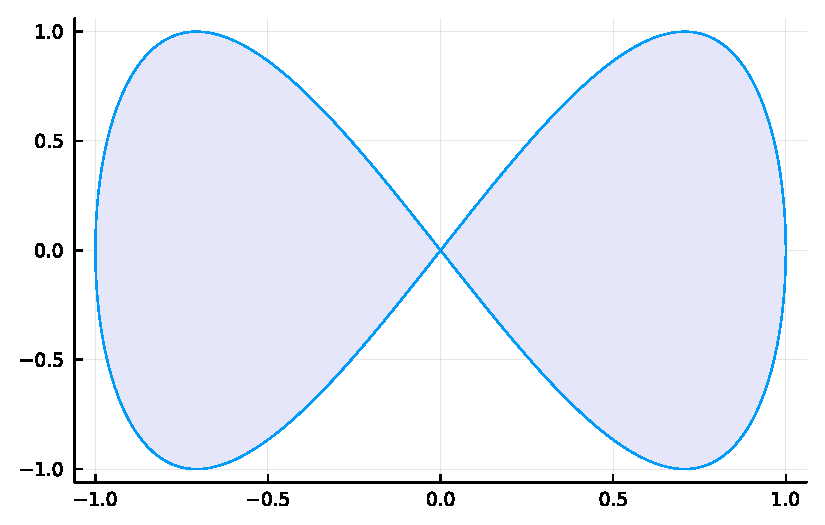
\includegraphics{QuartoBasics_files/mediabag/QuartoBasics_files/figure-pdf/fig-parametric-output-1.pdf}

}

\caption{\label{fig-parametric}Parametric Plots}

\end{figure}%

Quarto
ではこのような数式・コードが共存するドキュメントが,極めて簡単に+凡ゆるフォーマットで作成できる.

計算統計の研究をしている筆者にとっては何より,数式とコードが自然に共存する
PDF を簡単に書けること,そして自学のためのノートがそのまま HTML
としてブログの形で公開できることが,大変嬉しかった.

特に VSCode の拡張機能と組み合わせれば,RStudio
のような隙のない統合開発環境が得られる.\footnote{特に,VSCode
  では\href{https://quarto.org/docs/visual-editor/vscode/}{ビジュアルモードでの編集}もサポートされており,Jupyter
  Notebookと全く同じ使用感で始められる.}

基本的な仕組みとして,自分で作成するのは
\texttt{.qmd}ファイルのみである.

その後は\texttt{quarto\ render}コマンドにより,

\begin{tcolorbox}[enhanced jigsaw, bottomrule=.15mm, leftrule=.75mm, colframe=quarto-callout-important-color-frame, opacityback=0, toprule=.15mm, colback=white, arc=.35mm, breakable, rightrule=.15mm, left=2mm]

\begin{itemize}
\tightlist
\item
  コードブロックは Jupyter によって処理され,
\item
  全体は markdown に変換され,
\item
  Pandoc によって\texttt{pdf}, \texttt{html}, \texttt{word}
  など好きな形式に最終出力できる.
\end{itemize}

\end{tcolorbox}

拡張機能をオンにした VSCode
では\texttt{Run\ Cell}ボタンもあるので,ノートブック全体を毎度ビルドせずとも,コードブロックごとに実行して結果を見ることもできる.

\texttt{Ctrl+Enter} で1行ごとに実行できる操作感は \texttt{RStudio}
と同じである.

\subsubsection{美点}\label{ux7f8eux70b9}

\begin{tcolorbox}[enhanced jigsaw, bottomrule=.15mm, leftrule=.75mm, colframe=quarto-callout-tip-color-frame, opacityback=0, toprule=.15mm, colback=white, arc=.35mm, breakable, rightrule=.15mm, left=2mm]

\begin{itemize}
\tightlist
\item
  レンダリングがとんでもなく速い.体感で TeX の10分の1である.
\item
  それでいて数式とコードブロックを併在させることが出来る.なお,明かに
  TeX
  を意識していることがわかる使用感になっているし,\href{https://quarto.org/docs/books/}{本の作成も可能}としている.
\item
  (ちょっと使いにくい)ブラウザ上ではなく,好きなエディタで動く.Jupyter
  Notebook が続かない筆者にとって,この点は肝要である.
\item
  私用の勉強ノートとしても使えると同時に,内容そのままブログとして公開できる.
\item
  \href{https://quarto.org/docs/presentations/}{プレゼンテーションの作成にも使える}.
\item
  すごい細かいが,例えば \texttt{project\ type} を \texttt{website}
  としたリポジトリで\texttt{quarto\ render}をしても,不要なファイルが自動で削除される.このような点がライトユーザーでもとにかく使いやすい.
\item
  さらに\href{https://quarto.org/docs/interactive/}{インタラクティブな機能}を実現したブログを作ってみたい.
\end{itemize}

\end{tcolorbox}

\subsubsection{YAML Header}\label{yaml-header}

各ファイルの冒頭に YAML block
を用意することで,ノートブックの詳細を調整できる(参照:\href{https://quarto.org/docs/reference/formats/html.html}{HTML
Options}).

例えば本ページでは次のとおり:

\begin{Shaded}
\begin{Highlighting}[]
\PreprocessorTok{{-}{-}{-}}
\FunctionTok{title}\KeywordTok{:}\AttributeTok{ }\StringTok{"Quarto はじめて良かった"}
\FunctionTok{author}\KeywordTok{:}\AttributeTok{ }\StringTok{"司馬博文"}
\FunctionTok{date}\KeywordTok{:}\AttributeTok{ }\StringTok{"11/4/2023"}
\FunctionTok{date{-}modified}\KeywordTok{:}\AttributeTok{ }\StringTok{"7/7/2024"}
\FunctionTok{categories}\KeywordTok{:}\AttributeTok{ }\KeywordTok{[}\AttributeTok{Lifestyle}\KeywordTok{]}
\FunctionTok{abstract}\KeywordTok{:}\AttributeTok{ Quarto は TeX のような使用感で,数式とコードが併存する文章を書き,1つのソースファイルから PDF, HTML, Word, Reveal.js, PowerPoint などの多様な形式に出力できる次世代の執筆環境である.TeX, RStudio, Jupyter Notebook のいずれかに慣れている人であれば,極めて手軽に Quarto を使うことができる.}
\FunctionTok{abstract{-}title}\KeywordTok{:}\AttributeTok{ 概要}
\FunctionTok{format}\KeywordTok{:}
\AttributeTok{  }\FunctionTok{html}\KeywordTok{:}
\AttributeTok{    }\FunctionTok{mainfont}\KeywordTok{:}\AttributeTok{ }\StringTok{"Gill Sans"}
\AttributeTok{    }\FunctionTok{theme}\KeywordTok{:}\AttributeTok{ minty}
\AttributeTok{    }\FunctionTok{css}\KeywordTok{:}\AttributeTok{ assets/styles.css}
\AttributeTok{    }\FunctionTok{toc}\KeywordTok{:}\AttributeTok{ }\CharTok{true}
\AttributeTok{    }\FunctionTok{number{-}sections}\KeywordTok{:}\AttributeTok{ }\CharTok{true}
\AttributeTok{    }\FunctionTok{highlight{-}style}\KeywordTok{:}\AttributeTok{ ayu}
\AttributeTok{    }\FunctionTok{code{-}block{-}border{-}left}\KeywordTok{:}\AttributeTok{ }\StringTok{"\#7CC4AC"}
\AttributeTok{    }\FunctionTok{code{-}overflow}\KeywordTok{:}\AttributeTok{ scroll}
\AttributeTok{    }\FunctionTok{toc{-}title}\KeywordTok{:}\AttributeTok{ }\StringTok{"目次"}
\AttributeTok{    }\FunctionTok{abstract{-}title}\KeywordTok{:}\AttributeTok{ }\StringTok{"概要"}
\PreprocessorTok{{-}{-}{-}}
\end{Highlighting}
\end{Shaded}

\subsubsection{本文の書き方}\label{ux672cux6587ux306eux66f8ux304dux65b9}

\paragraph{数式}\label{ux6570ux5f0f}

本文は markdown 記法で書く.数式も使える:

\[
\operatorname{P}[\lvert\xi\rvert<t]\le2e^{-\frac{t^2}{2\sigma^2}},\qquad t>0.
\]

\paragraph{コード}\label{ux30b3ux30fcux30c9}

また,コードブロックにもコメントアウトと接頭辞の組み合わせ
\texttt{\#\textbar{}}
を前につけることでYAMLで指示が出せる(参照:\href{https://quarto.org/docs/reference/cells/cells-jupyter.html}{指示のリスト}).上のコードブロックには

\begin{Shaded}
\begin{Highlighting}[]
\CommentTok{\#| label: fig{-}polar}
\CommentTok{\#| fig{-}cap: "A line plot on a polar axis"}
\end{Highlighting}
\end{Shaded}

と追加されているために,出力された図にラベリングとキャプションが付いているのである.

\begin{Shaded}
\begin{Highlighting}[]
\ExtensionTok{pip3}\NormalTok{ install jupyter{-}cache}
\end{Highlighting}
\end{Shaded}

が必要であることに注意.

\subsubsection{カーネルの選択}\label{ux30abux30fcux30cdux30ebux306eux9078ux629e}

\begin{Shaded}
\begin{Highlighting}[]
\OperatorTok{\textgreater{}}\NormalTok{ python3 }\ExtensionTok{{-}m}\NormalTok{ venv GenAI}

\OperatorTok{\textgreater{}}\NormalTok{ source }\ExtensionTok{GenAI/bin/activate}
\end{Highlighting}
\end{Shaded}

により仮想環境を作成して入れるが,この環境を Jupyter notebook
で使うにはもう一手間必要である.

\begin{Shaded}
\begin{Highlighting}[]
\OperatorTok{\textgreater{}}\NormalTok{ pip }\FunctionTok{install}\NormalTok{ ipykernel}

\OperatorTok{\textgreater{}}\NormalTok{ python }\ExtensionTok{{-}m}\NormalTok{ ipykernel install }\AttributeTok{{-}{-}user} \AttributeTok{{-}{-}name}\OperatorTok{=}\NormalTok{GenAI}
\end{Highlighting}
\end{Shaded}

すると

\begin{Shaded}
\begin{Highlighting}[]
\ExtensionTok{jupyter}\NormalTok{ kernelspec list}
\end{Highlighting}
\end{Shaded}

により見つかるようになっている.YAML header で \texttt{jupyter:\ genai}
と指定すれば良い.

\subsection{Website の作り方}\label{website-ux306eux4f5cux308aux65b9}

\href{https://quarto.org/docs/publishing/github-pages.html}{公式 Guide}
を参考.

\subsubsection{\texorpdfstring{Source
Branchを\texttt{main}と別ける}{Source Branchをmainと別ける}}\label{source-branchux3092mainux3068ux5225ux3051ux308b}

まず\texttt{gh-pages}という全く新しいブランチを作成する.既存のリポジトリのコミット履歴とは独立している新しいブランチを作るときは\texttt{-\/-orphan}オプションが利用される.

\begin{codelisting}

\caption{\texttt{Terminal}}

\begin{Shaded}
\begin{Highlighting}[]
\FunctionTok{git}\NormalTok{ checkout }\AttributeTok{{-}{-}orphan}\NormalTok{ gh{-}pages}
\FunctionTok{git}\NormalTok{ reset }\AttributeTok{{-}{-}hard} \CommentTok{\# make sure all changes are committed before running this!}
\FunctionTok{git}\NormalTok{ commit }\AttributeTok{{-}{-}allow{-}empty} \AttributeTok{{-}m} \StringTok{"Initialising gh{-}pages branch"}
\FunctionTok{git}\NormalTok{ push origin gh{-}pages}
\FunctionTok{git}\NormalTok{ checkout main}
\end{Highlighting}
\end{Shaded}

\end{codelisting}

基本\texttt{gh-pages}ブランチには自分では立ち入らない.

\subsubsection{\texorpdfstring{\texttt{Publish}コマンドによるサイトの公開}{Publishコマンドによるサイトの公開}}\label{publishux30b3ux30deux30f3ux30c9ux306bux3088ux308bux30b5ux30a4ux30c8ux306eux516cux958b}

\texttt{main}ブランチにいることを確認して,

\begin{codelisting}

\caption{\texttt{Terminal}}

\begin{Shaded}
\begin{Highlighting}[]
\ExtensionTok{quarto}\NormalTok{ publish gh{-}pages}
\end{Highlighting}
\end{Shaded}

\end{codelisting}

を実行.

GitHubの方の設定\textbf{Settings:
Pages}で,Sourceを\texttt{gh-pages}ブランチの\texttt{/(root)}にしていることを確認すれば,これで無事サイトが公開されていることが確認できる.

\subsubsection{GitHub Action
の使用}\label{github-action-ux306eux4f7fux7528}

さらに,ローカル上で\texttt{render}するのではなく,コミットする度にGitHub上でレンダリングしてもらえるように自動化することもできる.こうするとスマホからも自分のサイトが更新できる.

まず,GitHubの設定の\textbf{Actions}セクションの\textbf{Workflow
permissions}から,読み書きの権限をGitHub Actionに付与する.

続いて,次の内容のファイルを\texttt{.github/workflows/publish.yml}に書き込む:

\begin{codelisting}

\caption{\texttt{.github/workflows/publish.yml}}

\begin{Shaded}
\begin{Highlighting}[]
\FunctionTok{on}\KeywordTok{:}
\AttributeTok{  }\FunctionTok{workflow\_dispatch}\KeywordTok{:}
\AttributeTok{  }\FunctionTok{push}\KeywordTok{:}
\AttributeTok{    }\FunctionTok{branches}\KeywordTok{:}\AttributeTok{ main}

\FunctionTok{name}\KeywordTok{:}\AttributeTok{ Quarto Publish}

\FunctionTok{jobs}\KeywordTok{:}
\AttributeTok{  }\FunctionTok{build{-}deploy}\KeywordTok{:}
\AttributeTok{    }\FunctionTok{runs{-}on}\KeywordTok{:}\AttributeTok{ ubuntu{-}latest}
\AttributeTok{    }\FunctionTok{permissions}\KeywordTok{:}
\AttributeTok{      }\FunctionTok{contents}\KeywordTok{:}\AttributeTok{ write}
\AttributeTok{    }\FunctionTok{steps}\KeywordTok{:}
\AttributeTok{      }\KeywordTok{{-}}\AttributeTok{ }\FunctionTok{name}\KeywordTok{:}\AttributeTok{ Check out repository}
\AttributeTok{        }\FunctionTok{uses}\KeywordTok{:}\AttributeTok{ actions/checkout@v4}

\AttributeTok{      }\KeywordTok{{-}}\AttributeTok{ }\FunctionTok{name}\KeywordTok{:}\AttributeTok{ Set up Quarto}
\AttributeTok{        }\FunctionTok{uses}\KeywordTok{:}\AttributeTok{ quarto{-}dev/quarto{-}actions/setup@v2}
\AttributeTok{        }\FunctionTok{with}\KeywordTok{:}
\AttributeTok{          }\FunctionTok{tinytex}\KeywordTok{:}\AttributeTok{ }\CharTok{true}\CommentTok{  \# https://github.com/quarto{-}dev/quarto{-}actions/tree/main/setup}
\AttributeTok{        }\FunctionTok{env}\KeywordTok{:}
\AttributeTok{          }\FunctionTok{GITHUB\_TOKEN}\KeywordTok{:}\AttributeTok{ $\{\{ secrets.GITHUB\_TOKEN \}\}}\CommentTok{  \# Setting GH\_TOKEN is recommended as installing TinyTeX will query the github API.}

\AttributeTok{      }\KeywordTok{{-}}\AttributeTok{ }\FunctionTok{name}\KeywordTok{:}\AttributeTok{ Render and Publish}
\AttributeTok{        }\FunctionTok{uses}\KeywordTok{:}\AttributeTok{ quarto{-}dev/quarto{-}actions/publish@v2}
\AttributeTok{        }\FunctionTok{with}\KeywordTok{:}
\AttributeTok{          }\FunctionTok{target}\KeywordTok{:}\AttributeTok{ gh{-}pages}
\CommentTok{          \# render: false  \# https://quarto.org/docs/publishing/github{-}pages.html\#additional{-}options}
\AttributeTok{        }\FunctionTok{env}\KeywordTok{:}
\AttributeTok{          }\FunctionTok{GITHUB\_TOKEN}\KeywordTok{:}\AttributeTok{ $\{\{ secrets.GITHUB\_TOKEN \}\}}
\end{Highlighting}
\end{Shaded}

\end{codelisting}

途中,\texttt{tinytex:\ true} とすることで,1つのページを HTML と pdf
の両方で閲覧可能になる.本ブログでは,\href{https://162348.github.io/static/CV/cv.html}{CV
のページ} でこの機能を使っている.

これで,\texttt{main}ブランチにコミットする度に,GitHub上で\texttt{render}が実行されることとなる.

\subsection{PDF の作り方}\label{pdf-ux306eux4f5cux308aux65b9}

\subsubsection{LuaLaTeX
を使う方法}\label{lualatex-ux3092ux4f7fux3046ux65b9ux6cd5}

LuaLaTeX を利用することで日本語を含んだ PDF を作成できる.

\begin{codelisting}

\caption{\texttt{report.qmd}}

\begin{Shaded}
\begin{Highlighting}[]
\NormalTok{title: "タイトル"}
\NormalTok{author: 司馬博文}
\NormalTok{date: 2023/12/11}
\NormalTok{format:}
\NormalTok{  pdf:}
\NormalTok{    toc: true}
\NormalTok{    number{-}sections: true}
\NormalTok{    urlcolor: minty}
\NormalTok{    template{-}partials: }
\NormalTok{      {-} ../../../assets/before{-}title.tex}
\NormalTok{    keep{-}tex: true}
\NormalTok{    block{-}headings: false}
\NormalTok{    pdf{-}engine: lualatex}
\NormalTok{    documentclass: ltjsarticle}
\end{Highlighting}
\end{Shaded}

\end{codelisting}

\paragraph{LuaLaTeX の注意}\label{lualatex-ux306eux6ce8ux610f}

\begin{Shaded}
\begin{Highlighting}[]
\FunctionTok{\textbackslash{}int}\NormalTok{\_\{}\FunctionTok{\textbackslash{}mathbb}\NormalTok{\{R\}\}}
\end{Highlighting}
\end{Shaded}

のような記法は,pdfLaTeX ではなぜかコンパイルが通るが,LuaLaTeX
(や殆どの pdfLaTeX 以外のエンジン)ではエラーになる.

\paragraph{LuaLaTeX の欠点}\label{lualatex-ux306eux6b20ux70b9}

\texttt{ltjsarticle} クラスでは

\begin{Shaded}
\begin{Highlighting}[]
\ExtensionTok{Font} \DataTypeTok{\textbackslash{}J}\NormalTok{Y3/mc/m/n/10=file:HaranoAjiMincho{-}Regular.otf:{-}kern}\KeywordTok{;}\VariableTok{jfm}\OperatorTok{=}\NormalTok{ujis }\ExtensionTok{at}\NormalTok{ 9.24713pt not loadable: metric data not found or bad.}
\OperatorTok{\textless{}}\NormalTok{to }\ExtensionTok{be}\NormalTok{ read again}\OperatorTok{\textgreater{}} 
\ExtensionTok{relax} 
\ExtensionTok{l.79} \DataTypeTok{\textbackslash{}k}\NormalTok{anjiencoding\{JY3\}}\DataTypeTok{\textbackslash{}s}\NormalTok{electfont}
                                 \ExtensionTok{\textbackslash{}adjustbaseline}
\end{Highlighting}
\end{Shaded}

というエラーが.一方で,\texttt{bxjsarticle} クラスでは

\begin{Shaded}
\begin{Highlighting}[]
\ExtensionTok{LaTeX}\NormalTok{ Error: File }\KeywordTok{\textasciigrave{}}\ExtensionTok{haranoaji.sty}\StringTok{\textquotesingle{} not found.}

\StringTok{Type X to quit or \textless{}RETURN\textgreater{} to proceed,}
\StringTok{or enter new name. (Default extension: sty)}

\StringTok{Enter file name: }
\StringTok{! Emergency stop.}
\StringTok{\textless{}read *\textgreater{}}
\end{Highlighting}
\end{Shaded}

というエラーが出る.

ローカルではインストールすれば良いだけであるが,これを GitHub Actions
上で実現する方法を考えあぐねていた.

\begin{tcolorbox}[enhanced jigsaw, colframe=quarto-callout-important-color-frame, opacityback=0, toprule=.15mm, colbacktitle=quarto-callout-important-color!10!white, breakable, title={注(TeX Live のアップデート方法)}, bottomrule=.15mm, leftrule=.75mm, opacitybacktitle=0.6, colback=white, arc=.35mm, coltitle=black, bottomtitle=1mm, toptitle=1mm, titlerule=0mm, rightrule=.15mm, left=2mm]

年度を跨いだ TeX Live manager
のアップデートは,次のようにする必要がある:

\begin{Shaded}
\begin{Highlighting}[]
\FunctionTok{wget}\NormalTok{ http://mirror.ctan.org/systems/texlive/tlnet/update{-}tlmgr{-}latest.sh}
\FunctionTok{chmod}\NormalTok{ +x update{-}tlmgr{-}latest.sh}
\FunctionTok{sudo}\NormalTok{ ./update{-}tlmgr{-}latest.sh}
\end{Highlighting}
\end{Shaded}

\end{tcolorbox}

\paragraph{LuaLaTeX
と日本語フォント}\label{lualatex-ux3068ux65e5ux672cux8a9eux30d5ux30a9ux30f3ux30c8}

なぜか

\begin{Shaded}
\begin{Highlighting}[]
\BuiltInTok{\textbackslash{}usepackage}\NormalTok{[haranoaji,nfssonly]\{}\ExtensionTok{luatexja{-}preset}\NormalTok{\}}
\end{Highlighting}
\end{Shaded}

で変わるのは英語文字だけである.

\paragraph{\texorpdfstring{\texttt{GitHub\ Actions}
の修正}{GitHub Actions の修正}}\label{github-actions-ux306eux4feeux6b63}

次のようにして,Set up Quarto と Render and Publish の間に,TinyTeX と
haranoaji.sty のインストールを使いすることで,GitHub
上でもレンダリングが可能になる.

\begin{codelisting}

\caption{\texttt{publish.yml}}

\begin{Shaded}
\begin{Highlighting}[]
\KeywordTok{{-}}\AttributeTok{ }\FunctionTok{name}\KeywordTok{:}\AttributeTok{ }\StringTok{\textquotesingle{}Install TinyTeX\textquotesingle{}}\CommentTok{  \# https://github.com/quarto{-}dev/quarto{-}actions/tree/main/setup}
\AttributeTok{  }\FunctionTok{env}\KeywordTok{:}
\AttributeTok{    }\FunctionTok{QUARTO\_PRINT\_STACK}\KeywordTok{:}\AttributeTok{ }\CharTok{true}
\AttributeTok{    }\FunctionTok{GITHUB\_TOKEN}\KeywordTok{:}\AttributeTok{ $\{\{ secrets.GITHUB\_TOKEN \}\}}\CommentTok{  \# Setting GH\_TOKEN is recommended as installing TinyTeX will query the github API.}
\FunctionTok{  run}\KeywordTok{: }\CharTok{|}
\NormalTok{    quarto install tool tinytex {-}{-}log{-}level warning}
\NormalTok{    case $RUNNER\_OS in }
\NormalTok{      "Linux")}
\NormalTok{          echo "$HOME/bin" \textgreater{}\textgreater{} $GITHUB\_PATH}
\NormalTok{          export PATH="$HOME/bin:$PATH"}
\NormalTok{          ;;}
\NormalTok{       "macOS")}
\NormalTok{          TLMGR\_PATH=$(dirname $(find \textasciitilde{}/Library/TinyTeX {-}name tlmgr))}
\NormalTok{          echo $TLMGR\_PATH \textgreater{}\textgreater{} $GITHUB\_PATH}
\NormalTok{          export PATH="$TLMGR\_PATH:$PATH"}
\NormalTok{          ;;}
\NormalTok{       "Windows")}
\NormalTok{          TLMGR\_PATH=$(dirname $(find $APPDATA/TinyTeX {-}name tlmgr.bat))}
\NormalTok{          echo $TLMGR\_PATH \textgreater{}\textgreater{} $GITHUB\_PATH}
\NormalTok{          export PATH="$TLMGR\_PATH:$PATH"}
\NormalTok{          ;;}
\NormalTok{        *)}
\NormalTok{          echo "$RUNNER\_OS not supported"}
\NormalTok{          exit 1}
\NormalTok{          ;;}
\NormalTok{    esac}
\NormalTok{    echo "TinyTeX installed !"}
\NormalTok{    tlmgr install haranoaji   \# Install haranoaji.sty}
\AttributeTok{  }\FunctionTok{shell}\KeywordTok{:}\AttributeTok{ bash}
\end{Highlighting}
\end{Shaded}

\end{codelisting}

\paragraph{ローカルの TinyTeX に haranoaji.sty
をインストールする方法}\label{ux30edux30fcux30abux30ebux306e-tinytex-ux306b-haranoaji.sty-ux3092ux30a4ux30f3ux30b9ux30c8ux30fcux30ebux3059ux308bux65b9ux6cd5}

\begin{Shaded}
\begin{Highlighting}[]
\ExtensionTok{tlmgr}\NormalTok{ install haranoaji}
\end{Highlighting}
\end{Shaded}

だと,すでに TeX Live
がローカルに存在する場合は,そちらにインストールされてしまう.

\begin{Shaded}
\begin{Highlighting}[]
\ExtensionTok{quarto}\NormalTok{ install tinytex}
\end{Highlighting}
\end{Shaded}

でインストールされる TinyTeX は,ホームディレクトリ下の
\texttt{\textasciitilde{}/Liberary/TinyTeX/}
にインストールされる.\footnote{MaxOS では.}

そこの,\texttt{tlmgr} がインストールされている場所まで行って,

\begin{Shaded}
\begin{Highlighting}[]
\ExtensionTok{tlmgr}\NormalTok{ install haranoaji}
\end{Highlighting}
\end{Shaded}

を実行すると良い.

だが,まだ見つからないと言われる\ldots\ldots{}

\begin{Shaded}
\begin{Highlighting}[]
\ExtensionTok{❯}\NormalTok{ ./tlmgr install haranoaji        }
\ExtensionTok{tlmgr:}\NormalTok{ package repository https://mirror.las.iastate.edu/tex{-}archive/systems/texlive/tlnet/ }\OperatorTok{(verified)}
\ExtensionTok{[1/1,} \PreprocessorTok{??}\NormalTok{:}\PreprocessorTok{??}\NormalTok{/}\PreprocessorTok{??}\NormalTok{:}\PreprocessorTok{??}\NormalTok{] install: haranoaji }\PreprocessorTok{[}\StringTok{25570k}\PreprocessorTok{]}
\ExtensionTok{running}\NormalTok{ mktexlsr ...}
\ControlFlowTok{done} \ExtensionTok{running}\NormalTok{ mktexlsr.}
\ExtensionTok{tlmgr:}\NormalTok{ package log updated: \textasciitilde{}/Library/TinyTeX/texmf{-}var/web2c/tlmgr.log}
\ExtensionTok{tlmgr:}\NormalTok{ command log updated: \textasciitilde{}/Library/TinyTeX/texmf{-}var/web2c/tlmgr{-}commands.log}
\end{Highlighting}
\end{Shaded}

\subsubsection{Typst
を用いる方法}\label{typst-ux3092ux7528ux3044ux308bux65b9ux6cd5}

\href{https://typst.app/}{HP}

使うフォントは次のように,\href{https://fonts.google.com/specimen/BIZ+UDPGothic}{Google
Fonts} を通じて,GitHub Actions 上でインストールすることもできるだろう:

\begin{Shaded}
\begin{Highlighting}[]
\FunctionTok{wget}\NormalTok{ https://github.com/google/fonts/raw/main/ofl/bizudpgothic/BIZUDPGothic{-}Regular.ttf}
\FunctionTok{wget}\NormalTok{ https://github.com/google/fonts/raw/main/ofl/bizudpgothic/BIZUDPGothic{-}Bold.ttf}
\end{Highlighting}
\end{Shaded}

typst の pdf
は数式の処理がまだ納得のいく設定が見つかっていないが,コードの扱いが非常に自然で,出来上がりも美しい.

ただし,事前に GitHub Actions
の環境上に対応する日本語フォントを用意しておく必要がある.

\texttt{\{yml\ filename="publish.yml"\}\ -\ name:\ Install\ Japanese\ Fonts\ \ \ env:\ \ \ \ \ GITHUB\_TOKEN:\ \$\{\{\ secrets.GITHUB\_TOKEN\ \}\}\ \ \#\ Setting\ GH\_TOKEN\ is\ recommended\ as\ installing\ TinyTeX\ will\ query\ the\ github\ API.\ \ \ run:\ \textbar{}\ \ \ \ \ git\ clone\ https://github.com/yuru7/udev-gothic.git\ \ \ \ \ cd\ udev-gothic\ \ \ \ \ sudo\ cp\ -r\ ./source\ /usr/share/fonts/truetype/udev-gothic\ \ \ \ \ sudo\ fc-cache\ -f\ -v}

\subsection{スライドの作り方}\label{ux30b9ux30e9ux30a4ux30c9ux306eux4f5cux308aux65b9}



\end{document}
